% !TEX root = main.tex

\begin{figure}[t]
\center
% \includegraphics[scale=1.]{figs/runtime_desktop_bpp_vienna_b2}
\begin{tabular}{cc}
\hspace{-4.5cm}{\panel{A}} & \hspace{-4.8cm}{\panel{B}} \\[-0.5cm]
\hspace{-.2cm}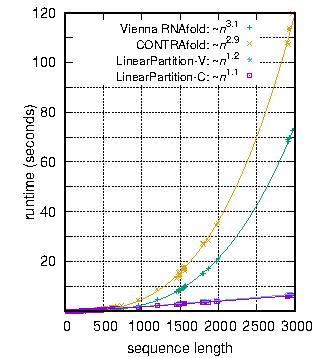
\includegraphics[scale=.9]{figs/runtime_desktop_overall_4sys_log_new}
&
\hspace{-.6cm}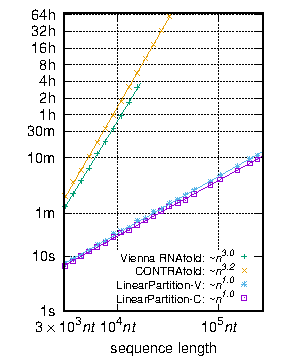
\includegraphics[scale=.9]{figs/rnacentral_desktop_runtime} \\[-1.8cm]
\hspace{-4.5cm}\raisebox{4.cm}{\panel{C}} & \hspace{-5.5cm}{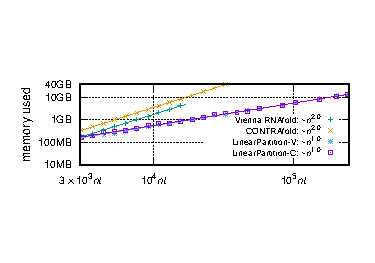
\includegraphics[scale=1.35]{figs/mem}} \\[-2.1cm]
% \multicolumn{2}{c}{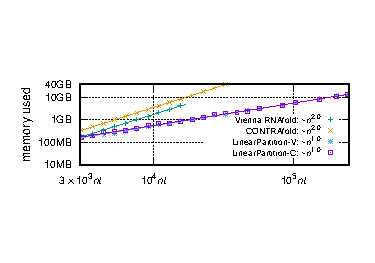
\includegraphics[scale=1.35]{figs/mem}} \\[-1.1cm]
\end{tabular}
\caption{Total runtime and memory usage of computing both the partition function and base pairing probabilities. % running speed and space comparisons.
% Runtime comparisons on ArchiveII and RNAcentral datasets, and memory usage comparison on RNAcentral dataset. 
{\bf A}: Runtime comparisons on the ArchiveII dataset; the curve-fittings were log-log in gnuplot with $n > 10^3$.
{\bf B}: Runtime comparisons on the RNAcentral dataset (log scale). %; the x-axis and y-axis are in log scale. 
%% Note that we show the total runtime of computing both the partition function and base pairing probabilities,
%% where the former takes about half of the time.
The partition function computation takes about half of the total time shown here.
% \viennarnafold overflows on the sequence of 19,071~\nts. 
% time limit is 24 hours.
{\bf C}: Memory usage comparisons on the RNAcentral dataset (log scale).
\label{fig:runtime}}
\vspace{-0.5cm}
\end{figure}
